\documentclass[11pt,a4paper]{report}
\usepackage[textwidth=37em,vmargin=30mm]{geometry}
\usepackage{calc,xunicode,amsmath,amssymb,paralist,enumitem,tabu,booktabs,datetime2,xeCJK,xeCJKfntef,listings}
\usepackage{tocloft,fancyhdr,tcolorbox,xcolor,graphicx,eso-pic,xltxtra,xelatexemoji}

\newcommand{\envyear}[0]{2025}
\newcommand{\envdatestr}[0]{2025-06-02}
\newcommand{\envfinaldir}[0]{webdb/2025/20250602/final}

\usepackage[hidelinks]{hyperref}
\hypersetup{
    colorlinks=false,
    pdfpagemode=FullScreen,
    pdftitle={Web Digest - \envdatestr}
}

\setlength{\cftbeforechapskip}{10pt}
\renewcommand{\cftchapfont}{\rmfamily\bfseries\large\raggedright}
\setlength{\cftbeforesecskip}{2pt}
\renewcommand{\cftsecfont}{\sffamily\small\raggedright}

\setdefaultleftmargin{2em}{2em}{1em}{1em}{1em}{1em}

\usepackage{xeCJK,xeCJKfntef}
\xeCJKsetup{PunctStyle=plain,RubberPunctSkip=false,CJKglue=\strut\hskip 0pt plus 0.1em minus 0.05em,CJKecglue=\strut\hskip 0.22em plus 0.2em}
\XeTeXlinebreaklocale "zh"
\XeTeXlinebreakskip = 0pt


\setmainfont{Brygada 1918}
\setromanfont{Brygada 1918}
\setsansfont{IBM Plex Sans}
\setmonofont{JetBrains Mono NL}
\setCJKmainfont{Noto Serif CJK SC}
\setCJKromanfont{Noto Serif CJK SC}
\setCJKsansfont{Noto Sans CJK SC}
\setCJKmonofont{Noto Sans CJK SC}

\setlength{\parindent}{0pt}
\setlength{\parskip}{8pt}
\linespread{1.15}

\lstset{
	basicstyle=\ttfamily\footnotesize,
	numbersep=5pt,
	backgroundcolor=\color{black!5},
	showspaces=false,
	showstringspaces=false,
	showtabs=false,
	tabsize=2,
	captionpos=b,
	breaklines=true,
	breakatwhitespace=true,
	breakautoindent=true,
	linewidth=\textwidth
}






\newcommand{\coverpic}[2]{
    % argv: itemurl, authorname
    Cover photo by #2~~(\href{#1}{#1})
}
\newcommand{\makeheader}[0]{
    \begin{titlepage}
        % \newgeometry{hmargin=15mm,tmargin=21mm,bmargin=12mm}
        \begin{center}
            
            \rmfamily\scshape
            \fontspec{BaskervilleF}
            \fontspec{Old Standard}
            \fontsize{59pt}{70pt}\selectfont
            WEB\hfill DIGEST
            
            \vfill
            % \vskip 30pt
            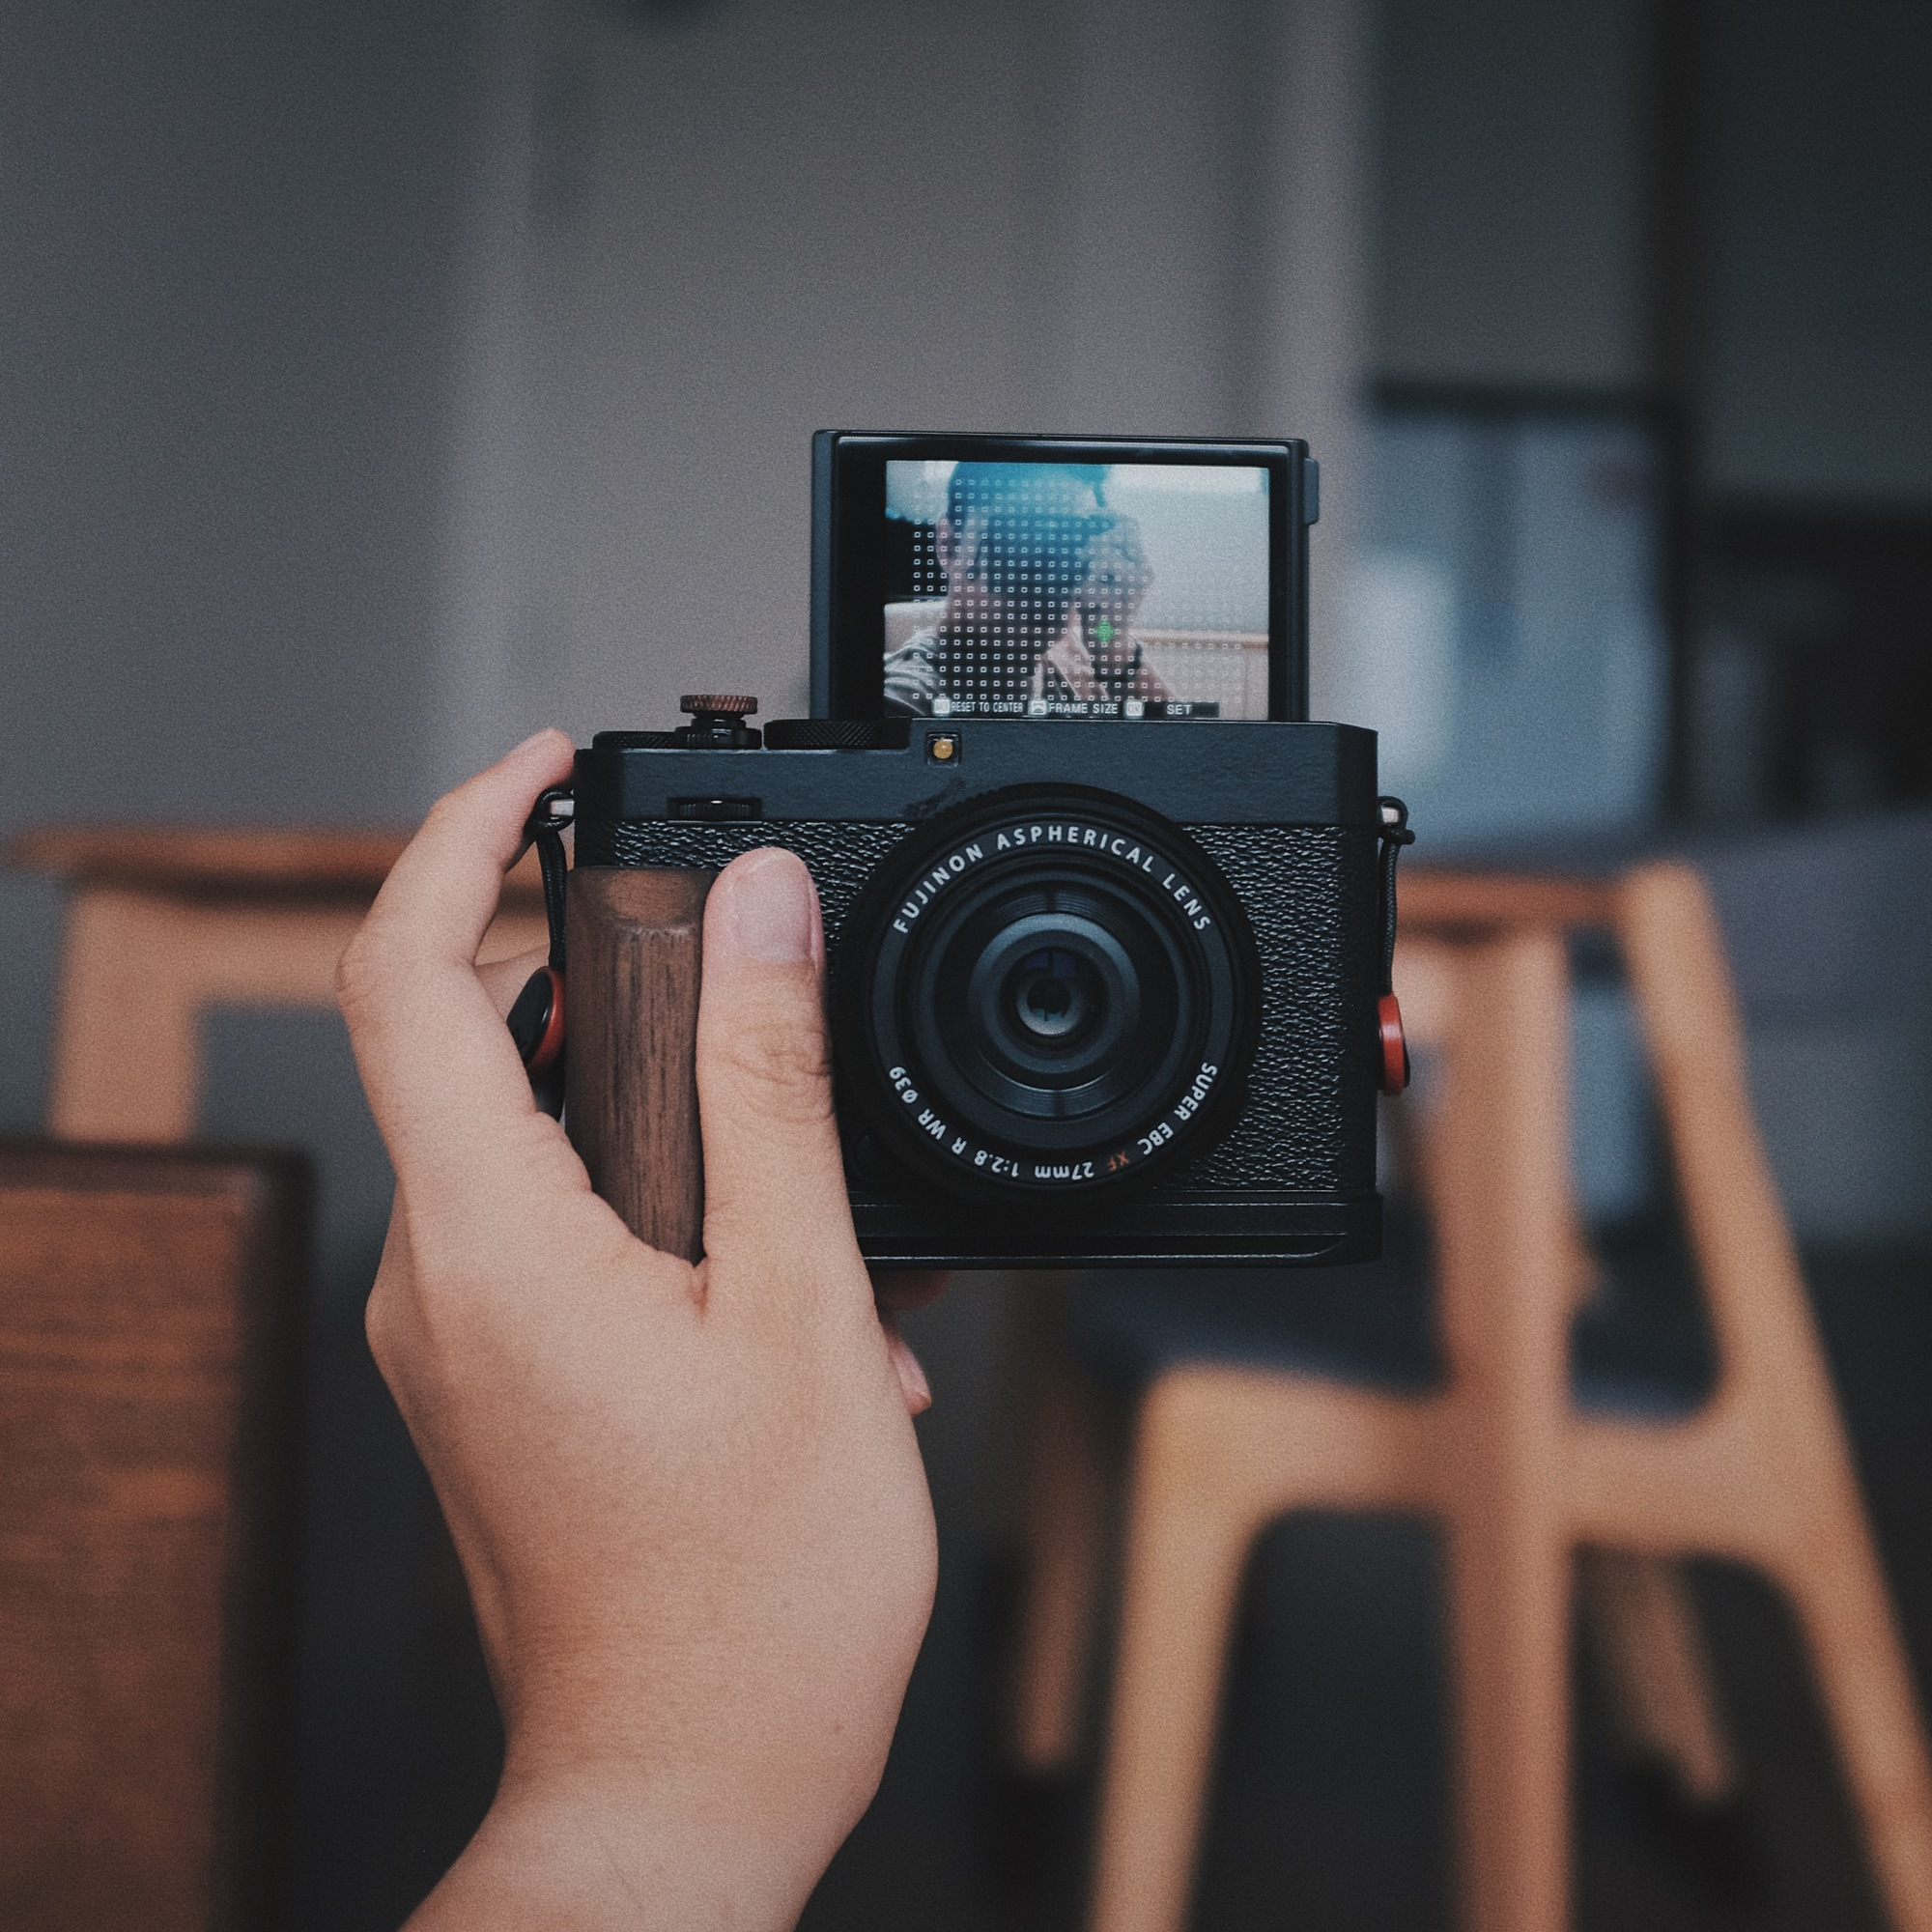
\includegraphics[width=\linewidth]{\envfinaldir/coverpic-prod.jpg}\par
            % \vskip 30pt
            \vfill

            \normalsize\rmfamily\scshape
            \copyright{} The Web Digest Project \hfill\large \envdatestr
        \end{center}
    \end{titlepage}
    % \restoregeometry
}
\newcommand{\simplehref}[1]{%
    \textcolor{blue!80!green}{\href{#1}{#1}}%
}
\renewcommand{\contentsname}{\center\Huge\sffamily\bfseries Contents\par\vskip 20pt}
\newcounter{ipartcounter}
\setcounter{ipartcounter}{0}
\newcommand{\ipart}[1]{
    % \vskip 20pt
    \clearpage
    \stepcounter{ipartcounter}
    \phantomsection
    \addcontentsline{toc}{chapter}{#1}
    % \begin{center}
    %     \Huge
    %     \sffamily\bfseries
    %     #1
    % \end{center}
    % \vskip 20pt plus 7pt
}
\newcounter{ichaptercounter}
\setcounter{ichaptercounter}{0}
\newcommand{\ichapter}[1]{
    % \vskip 20pt
    \clearpage
    \stepcounter{ichaptercounter}
    \phantomsection
    \addcontentsline{toc}{section}{\numberline{\arabic{ichaptercounter}}#1}
    \begin{center}
        \Huge
        \sffamily\bfseries
        #1
    \end{center}
    \vskip 20pt plus 7pt
}
\newcommand{\entrytitlefont}[1]{\subsection*{\raggedright\Large\sffamily\bfseries#1}}
\newcommand{\entryitemGeneric}[2]{
    % argv: title, url
    \parbox{\linewidth}{
        \entrytitlefont{#1}\par\vskip 5pt
        \footnotesize\ttfamily\mdseries
        \simplehref{#2}
    }\vskip 11pt plus 11pt minus 1pt
}
\newcommand{\entryitemGithub}[3]{
    % argv: title, url, desc
    \parbox{\linewidth}{
        \entrytitlefont{#1}\par\vskip 5pt
        \footnotesize\ttfamily\mdseries
        \simplehref{#2}\par\vskip 5pt
        \small\rmfamily\mdseries#3
    }\vskip 11pt plus 11pt minus 1pt
}
\newcommand{\entryitemAp}[3]{
    % argv: title, url, desc
    \parbox{\linewidth}{
        \entrytitlefont{#1}\par\vskip 5pt
        \footnotesize\ttfamily\mdseries
        \simplehref{#2}\par\vskip 5pt
        \small\rmfamily\mdseries#3
    }\vskip 11pt plus 11pt minus 1pt
}
\newcommand{\entryitemHackernews}[3]{
    % argv: title, hnurl, rawurl
    % \parbox{\linewidth}{
    %     \entrytitlefont{#1}\par\vskip 5pt
    %     \footnotesize\ttfamily\mdseries
    %     \simplehref{#3}\par
    %     \textcolor{black!50}{\href{#2}{#2}}
    % }\vskip 11pt plus 11pt minus 1pt
    \begin{minipage}{\linewidth}
            \entrytitlefont{#1}\par\vskip 5pt
            \footnotesize\ttfamily\mdseries
            \simplehref{#3}\par
            \textcolor{black!50}{\href{#2}{#2}}
    \end{minipage}\par\vskip 11pt plus 11pt minus 1pt
}







\begin{document}

\makeheader

\tableofcontents\clearpage




\ipart{Developers}
\ichapter{Hacker News}
\entryitemTwoLinks{M8.2 solar flare, Strong G4 geomagnetic storm watch}{https://news.ycombinator.com/item?id=44152154}{https://www.spaceweatherlive.com/en/news/view/581/20250531-m8-2-solar-flare-strong-g4-geomagnetic-storm-watch.html}

\entryitemTwoLinks{Root shell on a credit card terminal}{https://news.ycombinator.com/item?id=44150803}{https://stefan-gloor.ch/yomani-hack}

\entryitemTwoLinks{Ukraine destroys more than 40 military aircraft in drone attack deep in Russia}{https://news.ycombinator.com/item?id=44150789}{https://www.npr.org/2025/06/01/nx-s1-5419509/ukraine-destroys-military-aircraft-attack-inside-russia-planes}

\entryitemTwoLinks{Atari Means Business with the Mega ST}{https://news.ycombinator.com/item?id=44150002}{https://www.goto10retro.com/p/atari-means-business-with-the-mega}

\entryitemTwoLinks{Cinematography of ``Andor''}{https://news.ycombinator.com/item?id=44149718}{https://www.pushing-pixels.org/2025/05/20/cinematography-of-andor-interview-with-christophe-nuyens.html}

\entryitemTwoLinks{Canonicals Interview Process}{https://news.ycombinator.com/item?id=44149549}{https://dustri.org/b/my-experience-with-canonicals-interview-process.html}

\entryitemTwoLinks{Why DeepSeek is cheap at scale but expensive to run locally}{https://news.ycombinator.com/item?id=44149238}{https://www.seangoedecke.com/inference-batching-and-deepseek/}

\entryitemTwoLinks{Google AI Edge – On-device cross-platform AI deployment}{https://news.ycombinator.com/item?id=44149019}{https://ai.google.dev/edge}

\entryitemTwoLinks{Figma Slides Is a Beautiful Disaster}{https://news.ycombinator.com/item?id=44148933}{https://allenpike.com/2025/figma-slides-beautiful-disaster}

\entryitemTwoLinks{Father Ted Kilnettle Shrine Tape Dispenser}{https://news.ycombinator.com/item?id=44148853}{https://stephencoyle.net/kilnettle}

\entryitemTwoLinks{Structured Errors in Go (2022)}{https://news.ycombinator.com/item?id=44148734}{https://southcla.ws/structured-errors-in-go}

\entryitemTwoLinks{RenderFormer: Neural rendering of triangle meshes with global illumination}{https://news.ycombinator.com/item?id=44148524}{https://microsoft.github.io/renderformer/}

\entryitemTwoLinks{Stepping Back}{https://news.ycombinator.com/item?id=44147966}{https://rjp.io/blog/2025-05-31-stepping-back}

\entryitemTwoLinks{Progressive JSON}{https://news.ycombinator.com/item?id=44147945}{https://overreacted.io/progressive-json/}

\entryitemTwoLinks{Show HN: Patio – Rent tools, learn DIY, reduce waste}{https://news.ycombinator.com/item?id=44147803}{https://patio.so}

\entryitemTwoLinks{The NFS 4 Freezer Spacer In Science Fiction Sets}{https://news.ycombinator.com/item?id=44147631}{https://kolektiva.social/@beka\_valentine/114600567753999701}

\entryitemTwoLinks{New adaptive optics shows details of our star's atmosphere}{https://news.ycombinator.com/item?id=44147573}{https://nso.edu/press-release/new-adaptive-optics-shows-stunning-details-of-our-stars-atmosphere/}

\entryitemTwoLinks{YOLO-World: Real-Time Open-Vocabulary Object Detection}{https://news.ycombinator.com/item?id=44146858}{https://arxiv.org/abs/2401.17270}

\entryitemTwoLinks{Oniux: Kernel-level Tor isolation for any Linux app}{https://news.ycombinator.com/item?id=44146830}{https://blog.torproject.org/introducing-oniux-tor-isolation-using-linux-namespaces/}

\entryitemTwoLinks{CCD co-inventor George E. Smith dies at 95}{https://news.ycombinator.com/item?id=44146619}{https://www.nytimes.com/2025/05/30/science/george-e-smith-dead.html}\ichapter{Phoronix}
\entryitemGeneric{\hskip 0pt{}Wine 10.9 Released With EGL Support For All Graphics Drivers}{https://www.phoronix.com/news/Wine-10.9-Released}

\entryitemGeneric{\hskip 0pt{}Intel Overclocking Watchdog Driver Merged For Linux 6.16}{https://www.phoronix.com/news/Intel-Overclocking-Linux-6.16}

\entryitemGeneric{\hskip 0pt{}Linux 6.15 Shipped With A Nasty Power Regression For Some Systems}{https://www.phoronix.com/news/Linux-6.15-nosmt-Power-Regress}

\entryitemGeneric{\hskip 0pt{}Linux 6.16 Enables Support For Arm Scalable Matrix Extension "SME"}{https://www.phoronix.com/news/Linux-6.16-Restores-Arm-SME}

\entryitemGeneric{\hskip 0pt{}Apparent Git Scripting Issue Raised Concerns Of Possible Malicious Linux Kernel Activity}{https://www.phoronix.com/news/Linux-6.16-Git-Gone-Wrong}

\entryitemGeneric{\hskip 0pt{}FreeBSD 14.3 RC1 Brings OCI Images To Docker \& GitHub}{https://www.phoronix.com/news/FreeBSD-14.3-RC1-Released}

\entryitemGeneric{\hskip 0pt{}Snapdragon X Elite \& AMD's Grado + Strix Halo CPUs Captured Phoronix Reader Interest In May}{https://www.phoronix.com/news/Phoronix-May-2025}

\entryitemGeneric{\hskip 0pt{}OpenBMC 2.18 Released With Many More Motherboard Ports Upstreamed}{https://www.phoronix.com/news/OpenBMC-2.18-Released}

\entryitemGeneric{\hskip 0pt{}Linux 6.16 Now Enforces A Minimum Compiler Version Of GCC 8}{https://www.phoronix.com/news/Linux-6.16-Requires-GCC-8-Min}\ichapter{Dribbble}
\entryitemGeneric{\hskip 0pt{}Mnp Technologies - Logo Design}{https://dribbble.com/shots/26092034-Mnp-Technologies-Logo-Design}

\entryitemGeneric{\hskip 0pt{}Cre8tera // Website}{https://dribbble.com/shots/26091009-Cre8tera-Website}

\entryitemGeneric{\hskip 0pt{}Singular Logo Concept (Unused)}{https://dribbble.com/shots/26091755-Singular-Logo-Concept-Unused}

\entryitemGeneric{\hskip 0pt{}zeero logo design}{https://dribbble.com/shots/26087342-zeero-logo-design}

\entryitemGeneric{\hskip 0pt{}Shori Brand}{https://dribbble.com/shots/26088139-Shori-Brand}

\entryitemGeneric{\hskip 0pt{}Eagle}{https://dribbble.com/shots/26085536-Eagle}

\entryitemGeneric{\hskip 0pt{}Create email inbox composition}{https://dribbble.com/shots/26083118-Create-email-inbox-composition}

\entryitemGeneric{\hskip 0pt{}Roaring Bear}{https://dribbble.com/shots/26087788-Roaring-Bear}

\entryitemGeneric{\hskip 0pt{}Hand-drawn illustration pack}{https://dribbble.com/shots/26084735-Hand-drawn-illustration-pack}

\entryitemGeneric{\hskip 0pt{}B2B Dashboard \& Web App UI UX Design for Carbon Solutions}{https://dribbble.com/shots/26076624-B2B-Dashboard-Web-App-UI-UX-Design-for-Carbon-Solutions}

\entryitemGeneric{\hskip 0pt{}Apple}{https://dribbble.com/shots/26084067-Apple}

\entryitemGeneric{\hskip 0pt{}Patriot Logo Design (Unused for Sale)}{https://dribbble.com/shots/26081047-Patriot-Logo-Design-Unused-for-Sale}

\entryitemGeneric{\hskip 0pt{}Illustration}{https://dribbble.com/shots/26083223-Illustration}

\entryitemGeneric{\hskip 0pt{}Heliopoint}{https://dribbble.com/shots/26081987-Heliopoint}

\entryitemGeneric{\hskip 0pt{}Heyo Turns 2!}{https://dribbble.com/shots/26078572-Heyo-Turns-2}

\entryitemGeneric{\hskip 0pt{}Roaring Bear}{https://dribbble.com/shots/26077332-Roaring-Bear}

\entryitemGeneric{\hskip 0pt{}Smart Home App}{https://dribbble.com/shots/26076565-Smart-Home-App}

\entryitemGeneric{\hskip 0pt{}Fox Brand Mascot}{https://dribbble.com/shots/26077954-Fox-Brand-Mascot}

\entryitemGeneric{\hskip 0pt{}Europe Logo Concept}{https://dribbble.com/shots/26077297-Europe-Logo-Concept}

\entryitemGeneric{\hskip 0pt{}Game Studio Logo}{https://dribbble.com/shots/26076821-Game-Studio-Logo}

\entryitemGeneric{\hskip 0pt{}HYDRO - Logo Design}{https://dribbble.com/shots/26073470-HYDRO-Logo-Design}

\entryitemGeneric{\hskip 0pt{}Credit payment card bank app animation}{https://dribbble.com/shots/26063214-Credit-payment-card-bank-app-animation}

\entryitemGeneric{\hskip 0pt{}S}{https://dribbble.com/shots/26071612-S}

\entryitemGeneric{\hskip 0pt{}Dedicated to Dumplings}{https://dribbble.com/shots/26073310-Dedicated-to-Dumplings}


\ipart{Developers~~~~(zh-Hans)}
\ichapter{Solidot}
\entryitemGeneric{\hskip 0pt{}NASA 卫星确认火星溅射的证据}{https://www.solidot.org/story?sid=81441}

\entryitemGeneric{\hskip 0pt{}世界面临新形式的气候否认——经济不可行}{https://www.solidot.org/story?sid=81440}

\entryitemGeneric{\hskip 0pt{}越来越多的中国游戏公司开发单机游戏}{https://www.solidot.org/story?sid=81439}

\entryitemGeneric{\hskip 0pt{}天文学家发现以 44 分钟周期发射无线电波和 X 射线的神秘天体}{https://www.solidot.org/story?sid=81438}

\entryitemGeneric{\hskip 0pt{}印度严重的空气污染无意中起到了降温作用}{https://www.solidot.org/story?sid=81437}

\entryitemGeneric{\hskip 0pt{}白宫的健康报告被发现部分内容是大模型生成的}{https://www.solidot.org/story?sid=81436}

\entryitemGeneric{\hskip 0pt{}美国禁止向中国出售半导体设计软件}{https://www.solidot.org/story?sid=81435}

\entryitemGeneric{\hskip 0pt{}Stack Overflow 将测试付费给专家回答问题}{https://www.solidot.org/story?sid=81434}

\entryitemGeneric{\hskip 0pt{}SEC 撤销对币安的诉讼}{https://www.solidot.org/story?sid=81433}

\entryitemGeneric{\hskip 0pt{}全球气温到 2029 年可能首次升温超 2℃}{https://www.solidot.org/story?sid=81432}

\entryitemGeneric{\hskip 0pt{}研究人员认为大模型既不会思考也不会推理}{https://www.solidot.org/story?sid=81431}

\entryitemGeneric{\hskip 0pt{}惠普将停止在中国制造销往北美的产品}{https://www.solidot.org/story?sid=81430}

\entryitemGeneric{\hskip 0pt{}通过饮料摄入糖比食用糖对健康危害更大}{https://www.solidot.org/story?sid=81429}\ichapter{V2EX}
\entryitemGeneric{\hskip 0pt{}[NAS] infuse 最新版无法连上飞牛影视}{https://www.v2ex.com/t/1135786}

\entryitemGeneric{\hskip 0pt{}[问与答] macOS 虚拟显示器: DeskPad}{https://www.v2ex.com/t/1135785}

\entryitemGeneric{\hskip 0pt{}[Apple] ios 上有好用的能调 mcp 的 client 么}{https://www.v2ex.com/t/1135783}

\entryitemGeneric{\hskip 0pt{}[Apple] 你们的 Apple Device 最高电池循环数有多少?健康度又有多少?}{https://www.v2ex.com/t/1135782}

\entryitemGeneric{\hskip 0pt{}[问与答] 只有我这里的 google 变成这样了么}{https://www.v2ex.com/t/1135781}

\entryitemGeneric{\hskip 0pt{}[Go 编程语言] 有用 LiveKit 做过视频语音会议系统的没?}{https://www.v2ex.com/t/1135779}

\entryitemGeneric{\hskip 0pt{}[程序员] 2025 年了,传统分布式架构还会是主流吗}{https://www.v2ex.com/t/1135777}

\entryitemGeneric{\hskip 0pt{}[分享创造] 《菊与刀》:一个 AI 的终极感悟}{https://www.v2ex.com/t/1135776}

\entryitemGeneric{\hskip 0pt{}[Android] 闲鱼的开发程序员不是弱智}{https://www.v2ex.com/t/1135775}

\entryitemGeneric{\hskip 0pt{}[硬件] [求配置单] 1.5W-2W 纯游戏主机 (不含外设),追求性价比+战未来,求避坑指南!}{https://www.v2ex.com/t/1135773}

\entryitemGeneric{\hskip 0pt{}[分享创造] Komga 漫画服务器元数据刮削器}{https://www.v2ex.com/t/1135771}

\entryitemGeneric{\hskip 0pt{}[NAS] 绿联 dxp4800 安装黑群晖后老是自动重启}{https://www.v2ex.com/t/1135768}

\entryitemGeneric{\hskip 0pt{}[分享发现] 发现 HarmonyOS PC 自带了 Windows 虚拟机软件}{https://www.v2ex.com/t/1135767}

\entryitemGeneric{\hskip 0pt{}[问与答] 有没有一顿饭能买到的住宅 IP?}{https://www.v2ex.com/t/1135766}

\entryitemGeneric{\hskip 0pt{}[游戏] Discover Sprunki.lat – Free Online Music Creation Games for Everyone!}{https://www.v2ex.com/t/1135765}

\entryitemGeneric{\hskip 0pt{}[分享创造] 用 trae 开发了一个游戏,考验玩家极限能力,感觉 AI 编程还是有点东西的}{https://www.v2ex.com/t/1135763}

\entryitemGeneric{\hskip 0pt{}[前端开发] 一款更轻量、更自然,同时性能更强的前端框架}{https://www.v2ex.com/t/1135761}

\entryitemGeneric{\hskip 0pt{}[随想] 多看看宇宙题材相关的纪录片,人才能意识到自己有多渺小。}{https://www.v2ex.com/t/1135759}

\entryitemGeneric{\hskip 0pt{}[Java] 异步架构的设计困惑}{https://www.v2ex.com/t/1135758}

\entryitemGeneric{\hskip 0pt{}[WebRTC] 有用 LiveKit 开发过视频语音会议系统的嘛?}{https://www.v2ex.com/t/1135756}

\entryitemGeneric{\hskip 0pt{}[问与答] 你们有没有碰到过,那种突然感觉有点心慌,就像是心脏在喉咙口很明显跳两下的感觉}{https://www.v2ex.com/t/1135755}

\entryitemGeneric{\hskip 0pt{}[分享创造] 做了个在线挂机放置游戏,欢迎大家体验👏}{https://www.v2ex.com/t/1135754}

\entryitemGeneric{\hskip 0pt{}[问与答] emby 连接阿里云盘,哪个方案比较靠谱?}{https://www.v2ex.com/t/1135752}

\entryitemGeneric{\hskip 0pt{}[问与答] 关于有钱人家孩子升学问题}{https://www.v2ex.com/t/1135751}

\entryitemGeneric{\hskip 0pt{}[React] 有用 LiveKit 开发过视频语音会议系统的嘛}{https://www.v2ex.com/t/1135748}

\entryitemGeneric{\hskip 0pt{}[阅读] 有读过王东岳《物演通论》这本书的吗?}{https://www.v2ex.com/t/1135746}

\entryitemGeneric{\hskip 0pt{}[推广] Generate your essay titles with Essay Title Generator}{https://www.v2ex.com/t/1135744}

\entryitemGeneric{\hskip 0pt{}[全球工单系统] Cursor 这是啥情况啊?}{https://www.v2ex.com/t/1135743}

\entryitemGeneric{\hskip 0pt{}[旅行] 分享下自己定制的 9 天 8 晚西藏行程}{https://www.v2ex.com/t/1135742}

\entryitemGeneric{\hskip 0pt{}[MySQL] 《高性能 MySQL》第三版:是否已经过时?}{https://www.v2ex.com/t/1135741}

\entryitemGeneric{\hskip 0pt{}[健身] 不胖但是上腹有肉咋办}{https://www.v2ex.com/t/1135740}

\entryitemGeneric{\hskip 0pt{}[电动汽车] 为什么没有左脚刹车右脚油门的设计呢?}{https://www.v2ex.com/t/1135739}

\entryitemGeneric{\hskip 0pt{}[宽带症候群] 速报!安徽移动已开通``独立高清语音''!}{https://www.v2ex.com/t/1135738}

\entryitemGeneric{\hskip 0pt{}[投资] 又到了月末清算,晒一下上半年 5 个月在 IBKR 的收益}{https://www.v2ex.com/t/1135734}

\entryitemGeneric{\hskip 0pt{}[远程工作] 西安 招聘一位有区块链背景的 Java 后端 维护已有项目 需要有区块链开发基础 薪资 10k+}{https://www.v2ex.com/t/1135733}

\entryitemGeneric{\hskip 0pt{}[Telegram] telegram 机器人求推荐}{https://www.v2ex.com/t/1135732}

\entryitemGeneric{\hskip 0pt{}[问与答] 618 计划购入一个投影仪,坚果 N3 咋样}{https://www.v2ex.com/t/1135731}

\entryitemGeneric{\hskip 0pt{}[游戏] Found a Fascinating Music Creation Game Collection - Sprunki Green}{https://www.v2ex.com/t/1135729}

\entryitemGeneric{\hskip 0pt{}[健康] 赛博求医:我这种类型的喜欢吃甜食,是否属于正常?}{https://www.v2ex.com/t/1135727}

\entryitemGeneric{\hskip 0pt{}[分享创造] 终于等到您「熊猫健身 」2.0,全新升级来袭}{https://www.v2ex.com/t/1135721}

\entryitemGeneric{\hskip 0pt{}[硬件] B760M gaming wifi 和 14700F 合适吗}{https://www.v2ex.com/t/1135716}

\entryitemGeneric{\hskip 0pt{}[WireGuard] wg-easy 4 天前更新了,支持 IPV6 了。}{https://www.v2ex.com/t/1135715}

\entryitemGeneric{\hskip 0pt{}[分享创造] 学习做出海网站,开发+部署先尝试把流程跑通}{https://www.v2ex.com/t/1135714}

\entryitemGeneric{\hskip 0pt{}[程序员] 兄弟们, AI 开发工具到底用哪款, Azure AI Studio, AWS Bedrock, LangChain, LIamaIndex? 谢谢!}{https://www.v2ex.com/t/1135713}

\entryitemGeneric{\hskip 0pt{}[远程工作] 🚀 [远程招聘] PHP Laravel + Vue 全职开发工程师(日本项目,国内远程,不要求日语)}{https://www.v2ex.com/t/1135712}

\entryitemGeneric{\hskip 0pt{}[Rust] rust 来得快去得也快}{https://www.v2ex.com/t/1135711}

\entryitemGeneric{\hskip 0pt{}[问与答] Flutter dart 国内镜像源解决拉取依赖失败}{https://www.v2ex.com/t/1135709}

\entryitemGeneric{\hskip 0pt{}[生活] 今年 618 消费欲望不强,只买了一些生活必需品}{https://www.v2ex.com/t/1135708}

\entryitemGeneric{\hskip 0pt{}[分享发现] 用 ChatGPT 简单总结了一下《AI Engineering》这本书}{https://www.v2ex.com/t/1135705}

\entryitemGeneric{\hskip 0pt{}[职场话题] 仲裁的话, 2n 概率大吗}{https://www.v2ex.com/t/1135704}


\ipart{Generic News}







\clearpage
\leavevmode\vfill
\footnotesize

Copyright \copyright{} 2023-2025 Neruthes and other contributors.

This document is published with CC BY-NC-ND 4.0 license.

The entries listed in this newsletter may be copyrighted by their respective creators.

This newsletter is generated by the Web Digest project.

The newsletters are also delivered via Telegram channel \CJKunderline{\href{https://t.me/webdigestchannel}{https://t.me/webdigestchannel}}.\\
RSS feed is available at \CJKunderline{\href{https://webdigest.pages.dev/rss.xml}{https://webdigest.pages.dev/rss.xml}}.

This newsletter is available in PDF at
\CJKunderline{\href{https://webdigest.pages.dev/}{https://webdigest.pages.dev/}}.

The source code being used to generate this newsletter is available at\\
\CJKunderline{\href{https://github.com/neruthes/webdigest}{https://github.com/neruthes/webdigest}}.

This newsletter is also available in
\CJKunderline{\href{http://webdigest.pages.dev/readhtml/\envyear/WebDigest-20250602.html}{HTML}} and
\CJKunderline{\href{https://github.com/neruthes/webdigest/blob/master/markdown/\envyear/WebDigest-20250602.md}{Markdown}}.


\coverpic{https://unsplash.com/photos/books-are-arranged-neatly-on-a-wooden-bookshelf-DkLM7sDPzgA}{Brooke Balentine}


\end{document}
